\section{Introduction}

The {\em traveling salesman problem} (TSP) is a central problem in combinatorial optimization. Given a set $V$ of $n$ vertices and their pairwise distances, it asks for a Hamiltonian cycle of the minimum cost. In this paper, we study {\em sublinear time} algorithms for TSP. The algorithm is given query access to the distance pairs, and the goal is to estimate the solution cost in time sublinear in the input size (which is $\Theta(n^2)$).

TSP is NP-hard to approximate within a polynomial factor for an arbitrary distance function. As such, much of the work in the literature has been on more specific distance functions. Some notable examples include {\em graphic TSP} \cite{GharanSS11,MomkeS11,Mucha12,SeboV14,chen2020} where the distances are the shortest paths over an arbitrary unweighted undirected graph, {\em $(1, 2)$-TSP} \cite{AdamaszekMP18,chen2020,BermanK06,karp1972reducibility,MnichM18} where the distances are 1 or 2, and more generally {\em metric TSP} \cite{KarlinKG21,CzumajS-SIAM09,christofides1976worst,serdyukov1978nekotorykh} where the distances satsify triangle inequality. 

In 2003, \citet*{CzumajS-STOC04,CzumajS-SIAM09} showed that for any fixed $\epsilon > 0$, a $(1+\epsilon)$-approximation of the cost of metric minimum spanning tree (MST) and thus a  $(2+\epsilon)$-approximation of the cost of metric TSP can be found in $\widetilde{O}(n)$ time. Twenty years later, it still remains a major open problem to either break two-approximation in $n^{2-\Omega(1)}$ time or prove a lower bound.\footnote{See e.g. Open Problem 71 on \href{https://sublinear.info/index.php?title=Open_Problems:71}{sublinear.info} \cite{sublinear-info}.}
However, better bounds are known for both graphic TSP and $(1,2)$-TSP. In this paper, we present improved algorithms for these two well-studied variants of TSP. Our main tool to achieve this is an improved algorithm for the closely related {\em maximum path cover} problem which might be of independent interest.





\vspace{-0.2cm}
\paragraph{Maximum Path Cover:}  The maximum path cover in a graph is a collection of vertex disjoint paths with the maximum number of edges in it. The (almost) 1/2-approximate maximum matching size estimator of \citet*{behnezhad2021} immediately implies an (almost) 1/4-approximation for the maximum path cover problem in $\widetilde{O}(n)$ time.\footnote{The application of sublinear time maximum matching algorithms for approximating maximum path cover was first proposed by Gupta and Onak. See \cite{sublinear-info}.} This can be improved to an (almost) $(3/8 = .375)$-approximation using the {\em matching-pair} idea of \citet*{chen2020} in $\widetilde{O}(n \sqrt{n})$-time.\footnote{We note that even though a subsequent result of \citet*{behnezhad2021} improved the running time for maximal matchings and graphic TSP from $O(n\sqrt{n})$ in \cite{chen2020} to $\widetilde{O}(n)$, it is not immediately clear whether the same holds for path cover and $(1,2)$-TSP as they rely on a different notion of a matching pair.} Our first main contribution is an improvement over both of these results:

\begin{graytbox}
\begin{result}[Formally as \Cref{thm: disjoint-paths-algorithm}]\label{res:path-cover}
    For any $\epsilon > 0$, there is a randomized algorithm that w.h.p. $(1/2-\epsilon)$-approximates the size of maximum path cover in $\widetilde{O}(n \cdot \poly(1/\epsilon))$ time.
\end{result}
\end{graytbox}

Besides quantitavely improving prior work both in the running time and the approximation ratio, \cref{res:path-cover} reaches a qualitatively important milestone as well. First, the running time of \Cref{res:path-cover} is information-theoretically optimal up to $\poly\log n$ factors (the lower bound holds for any constant approximation --- see \cref{sec:hardness}). Second, its approximation ratio hits a rather important barrier. We give a non-trivial reduction that shows a $(1/2+\Omega(1))$-approximation in $\widetilde{O}(n)$ time for maximum path cover would imply the same bound for maximum matching in bipartite graphs. Such a result has remained elusive for matching, which is one of the most extensively studied problems in the literature of sublinear time algorithms. See \Cref{sec:lowerbound}.

It is also worth noting that in bounding the running time of our algorithm in \cref{res:path-cover}, we use connections to parallel algorithms. Such a connection was previously only used for matchings \cite{behnezhad2021}.

\setlength\extrarowheight{5pt}
\begin{center}
\begin{table}[ht]
\begin{tabular}{ | >{\centering\arraybackslash} m{7em} |  >{\centering\arraybackslash} m{10em}| >{\centering\arraybackslash} m{7em} | >{\centering\arraybackslash} m{14.3em} |}   
  \hline
  Running Time& Approximation Ratio & Metric & Reference\\ 
  \hline
   \hline
   $\widetilde{O}(n)$ & $1.75+\epsilon$ & (1,2) & Folklore\\
   \hline
   $\widetilde{O}(n\sqrt{n})$ & $1.625+\epsilon$ & (1,2) & \citet*{chen2020}\\
   \hline
   $\widetilde{O}(n)$ & $1.5+\epsilon$ & (1,2) & \textbf{This work} (\cref{res:12-TSP})\\
   \hline \hline
   $\widetilde{O}(n)$ & $1.929$ & Graphic & \citet*{chen2020}\\
   \hline
   $\widetilde{O}(n)$ & $1.834$ & Graphic & \textbf{This work} (\cref{res:graphicTSP})\\
   \hline
   $n^{2-\Omega(1)}$ & $1.667$ & Graphic & \textbf{This work} (\cref{res:graphicTSP2})\\
   \hline \hline
   $\Omega(n^2)$& $1 + \epsilon$ & (1,2) \& Graphic & \citet*{chen2020}\\
   \hline
   $n^{1+\Omega(1)}$ (Conditional) & $1.5 - \epsilon$  & (1,2) \& Graphic & \textbf{This work} (\Cref{cor:matching-via-12tsp})\\
   \hline
\end{tabular}
\captionsetup{justification=centering}
\caption{Comparison of running time and approximation ratio of our TSP algorithms and lower bounds with prior work.}
\label{tbl:comparision}
\end{table}
\end{center}


\vspace{-4em}
\paragraph{$(1,2)$-TSP:} The $(1,2)$-TSP problem has been studied extensively in the classical setting. In his landmark paper,  \citet*{karp1972reducibility} showed that $(1,2)$-TSP is NP-hard. \citet*{PapadimitriouY93} then proved its APX-hardness. Since then there has been a significant amount of work on $(1,2)$-TSP in the classical setting.  The current best known inapproximability bound for $(1, 2)$-TSP is 535/534 \cite{KarpinskiS12}. After a series of works, the best known polynomial time approximation is $8/7$ \cite{BermanK06} which can be implemented in $O(n^3)$ time \cite{AdamaszekMP18}. For sublinear time algorithms, an $\widetilde{O}(n)$-time (almost) $1.75$-approximation is folklore \cite{sublinear-info}. \citet*{chen2020} improved the approximation to (almost) $1.625$ in $\widetilde{O}(n\sqrt{n})$ time.

It is not hard to see that up to a small additive error of 1, $(1,2)$-TSP is equivalent to finding a maximum path cover on the weight-1 edges and then connecting their endpoints via weight-2 edges. A simple calculation shows that any $\alpha$-approximation for the maximum path cover problem leads to a $(2-\alpha)$-approximation for $(1,2)$-TSP. Our path cover algorithm of \Cref{res:path-cover} immediately implies the following result as a corollary:
\begin{graytbox}
\begin{result}\label{res:12-TSP}
    For any $\epsilon > 0$, there is a randomized algorithm that w.h.p. $(1.5+\epsilon)$-approximates the cost of $(1,2)$-TSP in $\widetilde{O}(n \cdot \poly(1/\epsilon))$ time.
\end{result}
\end{graytbox}

Similar to \Cref{res:path-cover}, the running time of \Cref{res:12-TSP} is information-theoretically optimal up to $\poly\log n$ factors, and its approximation ratio hits a natural barrier due to a connection to sublinear time matching that we establish in this work.

\paragraph{Graphic TSP:} The graphic TSP problem is equivalent to finding a tour of the minimium size that visits all the vertices. This is an important instance of TSP that has received a lot of attention over the years. For polynomial time algorithms, a $1.5$-approximation of \citet*{christofides1976worst} (which also works more generally for metric TSP) had remained the best known until a series of works over the last decade improved it to $(1.5 - \epsilon_0)$ \cite{GharanSS11}, $1.461$ \cite{MomkeS11}, $1.444$ \cite{Mucha12}, and finally to 1.4 \cite{SeboV14}. For sublinear time algorithms, \citet*{chen2020} showed that an (almost) $(27/14 \approx 1.928)$-approximation of graphic TSP can be obtained in $\widetilde{O}(n \sqrt{n})$ time. The running time was subsequently improved to $\widetilde{O}(n)$ by \citet*{behnezhad2021}.

We first show that plugging \cref{res:path-cover} into the framework of \cite{chen2020} immediately improves their approximation from $1.928$ to (almost) $1.9$ while keeping the running time $\widetilde{O}(n)$. We then give a more fine tuned algorithm that obtains a much improved approximation ratio of $(11/6 \approx 1.833)$.

\begin{graytbox}
\begin{result}\label{res:graphicTSP}
    For any $\epsilon > 0$, there is a randomized algorithm that w.h.p. $(1+\epsilon)(\frac{11}{6} \approx 1.833)$-approximates the cost of graphic TSP in $\widetilde{O}(n \cdot \poly(1/\epsilon))$ time.
\end{result}
\end{graytbox}


Over the past few years, significant advancements have been made in the development of sublinear matching algorithms. Several recent results \cite{BehnezhadRR23focs, behnezhadroghanirubinstein2022,brrstoc24, BehnezhadRRS-ArXiv22, bhattacharya2023dynamic, sayanSublinear2022} have led to the creation of a $(1, \epsilon n)$-approximation algorithm for maximum matching, with running time of $n^{2-\Omega_{\epsilon}(n)}$. Leveraging these sublinear algorithms, we have devised a slightly subquadratic algorithm that provides a more accurate estimation of the size of graphic TSP.


\begin{graytbox}
\begin{result}\label{res:graphicTSP2}
    For any $\epsilon > 0$, there is a randomized algorithm that w.h.p. $(1+\epsilon)(\frac{5}{3} \approx 1.666)$-approximates the cost of graphic TSP in $n^{2-\Omega_{\epsilon}(1)}$ time.
\end{result}
\end{graytbox}

We contrast our results with prior sublinear TSP algorithms in \Cref{tbl:comparision}.


\paragraph{Further related work:} Finally, we note that in a recent paper, \citet*{ChenMetric-Arxiv22} show that assuming that the metric has a spanning tree supported on weight 1 edges, one can obtain a $(2-\epsilon_0)$-approximation with $\widetilde{O}(n\sqrt{n})$ queries for some small unspecified constant $\epsilon_0 > 0$. While this is a more general metric than graphic TSP and (1,2)-TSP that we study in this paper, we note that the two papers are orthogonal and their results are incomparable. In particular, the techniques developed in this paper are specifically designed to improve the approximation to much below 2, whereas \cite{ChenMetric-Arxiv22} focuses on generalizing the distance function while beating 2.



\section{Technical Overview}\label{sec:techniques}

In this section, we give an overview of our algorithms, especially our sublinear time maximum path cover algorithm of \cref{res:path-cover} which is the key to the other results as well.


Let us start with using matchings to approximate maximum path cover. Consider a graph that has a Hamiltonian path. Here, the optimal maximum path cover has size $n-1$. On the other hand, any maximum matching can have at most $n/2$ edges, which is by a factor 2 smaller than our optimal path cover. On top of this, we only know close to 1/2 approximations for maximum matching if we restrict the running to be close to linear in $n$ \cite{behnezhad2021,BehnezhadRRS-ArXiv22}, thus can only achieve an approximation close to 1/4.

Instead of a single matching, \citet*{chen2020} showed how to estimate the number of edges in a {\em maximal matching pair} in $\widetilde{O}(n\sqrt{n})$ time, where a matching pair is simply two edge disjoint matchings. It is not hard to see that the number of edges in a maximal matching pair is at least half the number of edges in a maximum path cover. The problem, however, is that a maximal matching pair is not a collection of paths! In particular, the two matchings can form cycles of length as small as four. Therefore, one may only be able to use 3/4 fraction of the edges of a matching pair in a path cover. This is precisely why the algorithm of \cite{chen2020} only obtains a $\frac{1}{2} \times \frac{3}{4} = \frac{3}{8}$ approximation for path cover, and a $2-\frac{3}{8} = 1.625$ approximation for $(1,2)$-TSP.  

If we could modify the matching pair algorithm of \cite{chen2020}, and avoid cycles by manually excluding edges whose endpoints are the endpoints of a path in the current matching pair, then we could avoid the 3/4 factor loss discussed above and achieve a 1/2-approximation. Unfortunately, checking whether the endpoints of an edge are endpoints of a path requires knowledge about whether a series of other edges belong to the solution, which seems hard to implement in sublinear time. 

Instead of checking for cycles manually, we introduce the following \Cref{alg:path-cover11} which avoids cycles more naturally. While our final algorithm is a modified variant of \Cref{alg:path-cover11} described below, we start with \Cref{alg:path-cover11} as we believe it provides the right intuition.


\begin{algorithm}[H]
\caption{A new algorithm for path cover.}
\label{alg:path-cover11}

	Initialize $P \gets \emptyset$.
	
	Each vertex $v$ has two {\em ports} that we denote by $v^0$ and $v^1$. Each of these ports throughout the algorithm will be either {\em free} or {\em occupied}. Initially, all ports are free.
	
	Iterate over the edges in some ordering $\pi$. Upon visiting an edge $e=(u, v)$: 
	
	{
	\begin{itemize}[itemsep=-3pt,topsep=0pt,leftmargin=10pt]
	    \item If $v^0$ and $u^0$ are free, add $e$ to $P$, mark $v^0$ and $u^0$ as occupied, and skip to the next edge.
        \item If $v^1$ and $u^0$ are free, add $e$ to $P$, mark $v^1$ and $u^0$ as occupied, and skip to the next edge.
        \item If $v^0$ and $u^1$ are free, add $e$ to $P$, mark $v^0$ and $u^1$ as occupied, and skip to the next edge.
	\end{itemize}
	}
	
    Return $P$.
\end{algorithm}

Two properties of \Cref{alg:path-cover11} are crucial. First, it prioritizes occupying $(u^0, v^0)$ (compared to $(u^1, v^0)$ or $(u^0, v^1)$) which in particular implies that any component in $P$ must have a $(u^0, v^0)$ edge. Second, it never occupies $(u^1, v^1)$ with an edge $(u, v)$.  While it is easy to see that the output of \Cref{alg:path-cover11} has maximum degree 2, and is thus a collection of paths or cycles, the two properties above actually guarantee that it never includes any cycle. See \cref{fig:no-cycle}. We provide the formal proof of this later in \cref{sec:pathcover-algs}. Additionally, we show that the output of \Cref{alg:path-cover11} must be at least half the size of a maximum path cover, as we prove next. Hence, if we manage to estimate the size of the output $P$ of \Cref{alg:path-cover11}, then we have proved \Cref{res:path-cover}.

\begin{figure}[h]
    \centering
    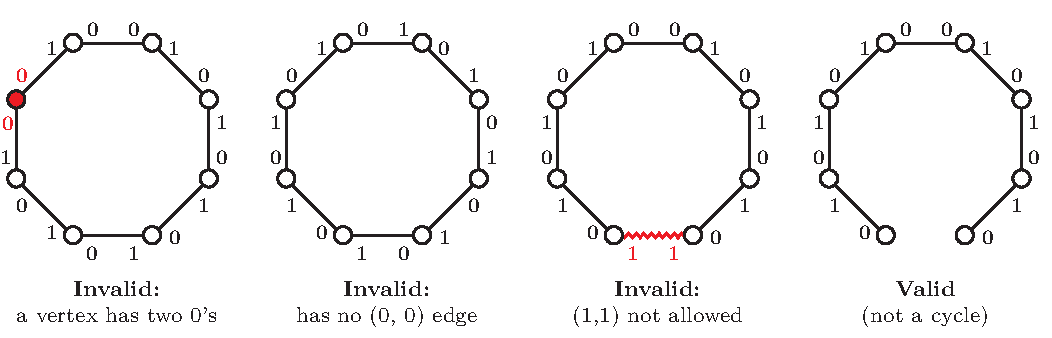
\includegraphics[scale=0.85]{fig/techniques.pdf}
    \caption{Examples of why the output of \Cref{alg:path-cover11} will not have cycles.}
    \label{fig:no-cycle}
\end{figure}

Our final algorithm is slightly different from \algone{} discussed above. In particular, we slightly relax it---see \algtwo{}---so that it can be solved via a randomized greedy maximal independent set (RGMIS), for which we have a rich toolkit of sublinear time estimators. Existing approaches (particularly the algorithm of \citet*{YoshidaYI09} and its two-step implementation by \citet*{chen2020}) can be employed to estimate the value of this modified \algtwo{} in $\widetilde{O}(n\sqrt{n})$ time. We achieve the improved, and near tight, $\widetilde{O}(n)$ time bound guarantee of \Cref{res:path-cover} by building on the analysis of \citet*{behnezhad2021} for maximal independent set on the line graphs (i.e., maximal matchings). Though we note that several new ideas are needed, because the MIS graph in our case will not be exactly a line graph. We defer more discussions about this to \cref{sec:pathcover-algs,sec:query-process}. 

\paragraph{Implications for TSP:} By having an $\alpha$-approximate maximum path cover algorithm, we immediately obtain a $(2-\alpha)$-approximation for $(1,2)$-TSP. Therefore, the algorithm above immediately proves \Cref{res:12-TSP} that we can (almost) $1.5$-approximate $(1,2)$-TSP in $\widetilde{O}(n)$ time. For our \Cref{res:graphicTSP} for graphic TSP, we first observe that our improved path cover algorithm can be employed to provide a better lower bound for the optimal TSP solution. This improves the 1.92-approximation of \cite{chen2020} as black-box to 1.9-approximation (\cref{sec:graphic-TSP-minor}). However, the final improvement to 1.83 requires more ideas, in particular, on how to better estimate the number of certain {\em bridges} in the graph. See \cref{sec:graphic-TSP-major} for more details about this.


% \clearpage

\section{Preliminaries}

\paragraph{Problem Definition:} In the sublinear TSP problem, we have a set $V$ of $n$ vertices and a distance function $d: V \times V \to \mathbb{R}_+$. The algorithm has query access to this distance function. Namely, for any pair $(u, v)$ of the vertices of its choice, the algorithm may query the value of $d(u, v)$. The goal is to design an algorithm that runs in sublinear time in the input size, which is $\Theta(n^2)$ (all the distance pairs), and produces an estimate of the size of the optimal TSP solution. Denoting the optimal TSP value by $\tspsize{V}$, we say an estimate $\widetilde{\tau}(V)$ provides an $\alpha$-approximation for $\alpha \geq 1$ if
$$
    \tspsize{V} \leq \widetilde{\tau}(V) \leq \alpha \cdot \tspsize{V}.
$$
We focus specifically on {\em graph TSP} and {\em $(1,2)$-TSP} problems. In graphic TSP, the distance function $d$ is the shortest path metric on an unweighted undirected graph $G$ that is unknown to the algorithm. Note, however, that the distance queries essentially provide {\em adjacency matrix} access to this graph $G$. In $(1,2)$-TSP, the assumption is that $d(u, v) \in \{1,2\}$ for every pair $u, v$. In the case of $(1,2)$-TSP we may use $G$ to refer to the subgraph induced on the pairs with distance 1.

Defining graph $G$ as above, we use $n$ to denote the number of its vertices, $m$ to denote the number of its edges, $\Delta$ to denote its maximum degree, $\mu(G)$ to denote its maximum matching size, $\nu(G)$ to denote its minimum vertex cover size, and $\bar{d}$ to denote its average degree.

\paragraph{Path Cover Definitions:} Given an unweighted graph $G$, a path cover in $G$ is a collection of vertex disjoint paths in $G$. A maximum path cover is a path cover of $G$ with the maximum number of edges in it (note that we are not counting the number of paths, but rather the total number of edges in them). We use $\pathcoversize{G}$ to denote the size of the maximum path cover in $G$. We say an estimate $\widetilde{\rho}(G)$ for $\pathcoversize{G}$ provides an $(\alpha, \epsilon)$-approximation for $\alpha, \epsilon \in [0, 1]$ if
$$
    \alpha \cdot \pathcoversize{G} - \epsilon n \leq \widetilde{\rho}(G) \leq \pathcoversize{G}.
$$
We may also use $\alpha$-approximation instead of $(\alpha, 0)$-approximation.

\paragraph{Graph Theory Definitions/Tools:} A {\em bridge (cut edge)} in a graph is an edge whose deletion increases the number of connected components. Similarly, a {\em cut vertex} is a vertex whose deletion (along with its edges)  increases the number of connected components. A {\em biconnected graph} is a connected graph with no cut vertex. Also, a {\em biconnected component (block)} of a graph is a maximal biconnected subgraph of the original graph. A non-trivial biconnected component is a block that is not a bridge. We say a graph is {\em 2-edge-connected} if there is no bridge in the graph. A {\em 2-edge-connected component} of a graph is maximal 2-edge-connected subgraph of the original graph. The {\em bridge-block tree} of a graph is a tree obtained by contracting the 2-edge-connected components; note that the edge set of a bridge-block tree correspond to the bridges in the original graph.


We use the following classic theorem of K\"{o}nig \cite{Konig1916} that the size of the minimum vertex cover is equal to the size of maximum matching in bipartite graphs. Namely:

\begin{proposition}[K\"{o}nig’s Theorem]\label{prop:konig}
    In any bipartite graph $G$,  $\mu(G) = \nu(G)$.
\end{proposition}


\paragraph{Probabilistic Tools:} In our proofs, we use the following standard concentration inequalities.

\begin{proposition}[Chernoff Bound]\label{prop:chernoff}
    Let $X_1, X_2, \ldots, X_n$ be independent Bernoulli random variables. Let $X = \sum_{i=1}^{n} X_i$. For any $t > 0$, 
    $\Pr[|X - \E[X]| \geq t] \leq 2\exp\left(-\frac{t^2}{3\E[X]}\right).$
\end{proposition}

\begin{proposition}[Hoeffding’s Inequality]\label{prop:hoeffding}
    Let $X_1, X_2, \ldots, X_n$ be independent random variables such that $a \leq X_i \leq b$. Let $\bar{X} = (\sum_{i=1}^n X_i)/n$. For any $t > 0$, 
    $
    \Pr[|\bar{X} - \E[X]| \geq t] \leq 2\exp\left(-\frac{2nt}{(b-a)^2}\right).
    $
\end{proposition}



\section{New Meta Algorithms for Maximum Path Cover}\label{sec:pathcover-algs}

In this section, we present a new meta algorithm for maximum path cover that obtains a $1/2$-approximation. The algorithm, as we will state it in this section, will not be particularly in the sublinear time model. We discuss its sublinear time implementation later in \Cref{sec:query-process,sec: disjoint-paths-estimate}.

Our starting point is the \algone{} described in \cref{sec:techniques}. Let us first formally prove that it obtains a $1/2$-approximation, and that no component in it is a cycle.



\begin{claim}
    The output of \algone{} is a collection of disjoint paths.
\end{claim}
\begin{myproof}
    Since $P$ has maximum degree two, it suffices to show none of its connected components are cycles.  Property $(i)$  above implies that at any point during the algorithm, any degree one vertex $v$ has its port $v^0$ occupied. Now take an edge $e=(u, v)$ that forms a cycle if added to $P$. Both $u$ and $v$ must have degree one and so $u^0$ and $v^0$ are occupied. Since by property $(ii)$ edge $e$ does not occupy both $v^1$ and $u^1$, the algorithm does not add $e$ to $P$ thus not completing a cycle.
\end{myproof}

\begin{claim}\label{clm: alg-one-approx}
    Let $P^\star$ be {\em any} path cover using weight one edges. Then the output of \algone{} has size at least $\frac{1}{2}|P^\star|$.
\end{claim}
\begin{myproof}
    For any edge $e=(u, v) \in P^\star$ define $\phi(e) = \frac{1}{4}(\deg_P(u) + \deg_P(v))$. We first claim that for every edge $e=(u, v)$ in $G$, we have $\phi(e) \geq 1/2$ (or, equivalently, $\deg_P(u)+\deg_P(v) \geq 2$). This is clear for edges $e \in P$ due to the contribution of $e$ itself to its endpoints' degrees, so fix $e \not\in P$. Consider the time that we process $e=(u, v)$ in the algorithm and decide not to add it to $P$. We claim that out of $v^0, v^1, u^0, u^1$ at least two ports must be occupied. Suppose w.l.o.g. and for contradiction that only $v^x$ is occupied for $x \in \{0, 1\}$. Then $(u, v)$ can occupy $v^{1-x}$ and $u^x$ and be added to $P$. This contradicts $(u, v)$ not being added to $P$ and proves our claim that $\phi(e) \geq 1/2$. 
    
    From the discussion above, we get that
    $$
        \sum_{e \in P^\star} \phi(e) \geq \sum_{e \in P^\star} 1/2 = |P^\star|/2.
    $$
    
    Moreover, because every vertex has degree at most two in $P^\star$, we get 
    $$
    \sum_{e \in P^\star} \phi(e) = \frac{1}{4} \sum_{(u, v) \in P^\star} \deg_P(u)+\deg_P(v) \leq \frac{1}{4} \cdot 2 \sum_{v \in V} \deg_P(v) = |P|.
    $$
    
    The two inequalities above combined imply that $|P| \geq |P^\star|/2$.
\end{myproof}

As discussed, our final algorithm is different from \algone{} discussed above. One problem with \algone{} is that it cannot be cast as an instance of the randomized greedy maximal independent set (RGMIS) algorithm for which there is a rich toolkit of sublinear time estimators. To remedy this, we present a modified variant of \algone{} whose output is (almost) as good, but in addition can be modeled as an instance of RGMIS. We denote the output of RGMIS on a graph $G$ with a permutation $\pi$ on its vertices by $\RGMIS(G, \pi)$.

The algorithm is stated below as \algtwo{}. Similar to the output of \algone{}, the output of \algtwo{} can be verified to have maximum degree two. Thus, it is a collection of paths and cycles. But unlike \algone{}, the output of \algtwo{} can have cycles. This happens since, unlike \algone{}, each connected component of the output of \algtwo{} is not guaranteed to have an edge $(u, v)$ occupying both $u^0$ and $v^0$. Nonetheless, we are able to show that this bad event only happens for a small fraction of connected components of the output of \algtwo{} in expectation, and so once we remove one edge of each of these cycles, the resulting collection of disjoint paths has almost the same size.

\begin{algorithm}[H]
\caption{A modification of \algone{} that uses RGMIS.}
\label{alg:path-cover22}

\textbf{Parameter:} $K$ (think of it as a large constant integer).

Let $G=(V, E)$ be the subgraph of weight one edges. We construct a graph $H=(V_H, E_H)$ from $G$ on which we run RGMIS.
    
Each vertex in $H$ corresponds to an edge $e$ in $G$ and two {\em ports} (as in \algone{}) of the endpoints of $e$ that it occupies. Formally, for any $(u, v) \in E$ we have $K + 2$ vertices in $H$:
{
    \begin{itemize}[itemsep=-2pt,topsep=2pt]
        \item One vertex that corresponds to occuping $u^0$ and $v^1$.
        \item One vertex that corresponds to occuping $u^1$ and $v^0$.
        \item $K$ vertices that each corresponds to occuping $u^0$ and $v^0$.
    \end{itemize}
}

    
Consider two distinct vertices $a$ and $b$ in $H$ corresponding to edges $e_a$ and $e_b$ in $G$:
  
{ 
\begin{itemize}[itemsep=-2pt,topsep=2pt]
        \item If $e_a = e_b$ then we add an edge between $a$ and $b$ in $H$.
        \item If $e_a$ and $e_b$ share exactly one endpoint $v$ and both $a$ and $b$ occupy the same port of $v$, we add an edge between $a$ and $b$ in $H$.
    \end{itemize}
}
    
Find a randomized greedy maximal independent set $I$ of $H$.
    
Let $P$ be the set of edges in $G$ corresponding to the vertices in $I$.
    
Return $P$.


\end{algorithm}


\begin{observation}\label{obs:no-zero-cycle}
Let $C$ be a connected component in the output of \algtwo{}. If $C$ is a cycle, then every edge in $C$ occupies one 0-port and one 1-port (that is, no edge occupies two 0-ports).
\end{observation}
\begin{myproof}
    Suppose that $C$ has $n'$ vertices. Since each vertex in a cycle has degree two, both ports of each vertex in $C$ must be occupied. Hence, $n'$ 0-ports and $n'$ 1-ports of $C$ are occupied in total. Given that any edge occupies at least one 0-port by the algorithm, we cannot have an edge that occupies two 0-ports, or else we should occupy more 0-ports than 1-ports of $C$, which is a contradiction.
\end{myproof}

Next, we show that up to a factor of $(1+2/k)$ which is negligible for $K$ in the order $1/\epsilon$, the output of \algtwo{} is an (almost) 1/2-approximation of the maximum path cover value.

\begin{observation}\label{obs:one-zero-path}
Let $C$ be a connected component in the output of \algtwo{}. If $C$ is a path, then it contains at most one edge that occupies two 0-ports.
\end{observation}
\begin{myproof}
    Let $C$ be the path $(v_1, v_2, \ldots, v_r)$. Since the degree of any vertex $v_i$ for $1<i<r$ is two in the path, both ports of $v_i$ must be occupied. For $v_1$ and $v_r$, on the other hand, only one port is occupied. Hence, the total number of 0-ports that are occupied by $C$ minus the number of 1-ports occupied by it is at most two. This means that there is at most one edge that occupies two 0-ports since all other types of edges occupy exactly one 0-port and one 1-port.
\end{myproof}



\begin{lemma}\label{clm: approximation-bound}
let $P$ be the output of \algtwo{} on graph $G$. Then
$$
    \frac{1}{2} \rho(G) \leq \E|P| \leq \left(1+\frac{2}{K}\right) \rho(G),
$$
where the expectation is taken over the randomization of computing RGMIS in \algtwo{}.
\end{lemma}
\begin{proof}
    Let $P^*$ be a maximum path cover. For any edge $e=(u, v) \in P^\star$ define $\phi(e) = \frac{1}{4}(\deg_P(u) + \deg_P(v))$. With the exact same argument as in the proof of \Cref{clm: alg-one-approx}, we get that $\phi(e) \geq 1/2$, which implies
    \begin{align*}
        \sum_{e \in P^\star} \phi(e) \geq \sum_{e \in P^\star} 1/2 = \rho(G)/2.
    \end{align*}
    Since the degree of each vertex in $P$ is at most two, we get
    \begin{align*}
        \sum_{e \in P^\star} \phi(e) = \frac{1}{4} \sum_{(u, v) \in P^\star} \deg_P(u)+\deg_P(v) \leq \frac{1}{4} \cdot 2 \sum_{v \in V} \deg_P(v) = |P|.
    \end{align*}
    By combining above inequalities we get $ \frac{1}{2} \rho(G) \leq |P|$. Note that we do not need the randomization for the proof of the lower bound.
    
    By construction of $P$, every vertex has degree at most two in $P$. Hence, all connected components of $P$ are cycles and paths. We claim that at most $\frac{2}{K+2}$ fraction of connected components are cycles in expectation. Since the expected number of connected components is at most $\E|P|$, from this we get that the expected number of cycles is at most $2\E|P|/(K+2)$. By removing one edge from each cycle, we obtain a valid solution for maximum path cover problem. Thus,
    \begin{align*}
        \E|P| - \frac{2\E|P|}{K + 2} = \frac{K}{K+2} \E|P| \leq \rho(G) \qquad \Rightarrow \qquad \E|P| \leq \left(1+ \frac{2}{K}\right)\cdot\rho(G).
    \end{align*}
   
    So it remains to show that at most $\frac{2}{K+2}$ fraction of connected components are cycles in expectation. As we process edges one by one according to the ordering of RGMIS, let $A$ be the set of edges that none of their incident edges are added to the solution of \algtwo{}. By definition of $A$, if one copy of edge $(u, v)$ is in $A$, then all other copies of $(u,v)$ are also in $A$. Therefore, at any point during running RGMIS, if a new component is added to the solution, the edge $(u,v)$ that gets added to the solution occupies $(u^0, v^0)$ with probability at least $\frac{K}{K+2}$ since $K$ copies out of the $K+2$ copies are for $(u^0, v^0)$. Let $C_0$ be the number of times that the newly added component is an edge occupying two 0-ports, and $C_1$ be the number of times that the newly added component is an edge occupying one 0-port and one 1-port. By the above argument, we have
    \begin{align}\label{eq:cycle-ineq}
        \frac{\E[C_0]}{\E[C_0] + \E[C_1]} = \frac{K}{K+2}.
    \end{align}
    
    Note that after running \algtwo{}, it is possible that the number of connected components is actually smaller than $C_0 + C_1$, since some of the components may merge as the algorithm proceeds. However, by \Cref{obs:one-zero-path}, two components that their first edge occupies two 0-ports will not merge together. Also, by \Cref{obs:no-zero-cycle}, none of the cycle components have an edge that occupies two 0-ports. Therefore, in the end, there exists at most $\E[C_0] + \E[C_1]$ connected components and at least $\E[C_0]$ of them will not be cycles. This completes the proof.
    \end{proof}



% \clearpage
